\part{Fazit und Ausblick}

\begin{frame}
    \partpage
\end{frame}

\section{Fazit}

\begin{frame}{Fazit}
    \pageText{
        OR-Tools \par
        \large Hülle Fixieren\\
        Kanten Fixieren\\
        alternative Kantenbedingung
    }
\end{frame}

\begin{frame}{Fazit}
   \begin{figure}[h]
    \centering
    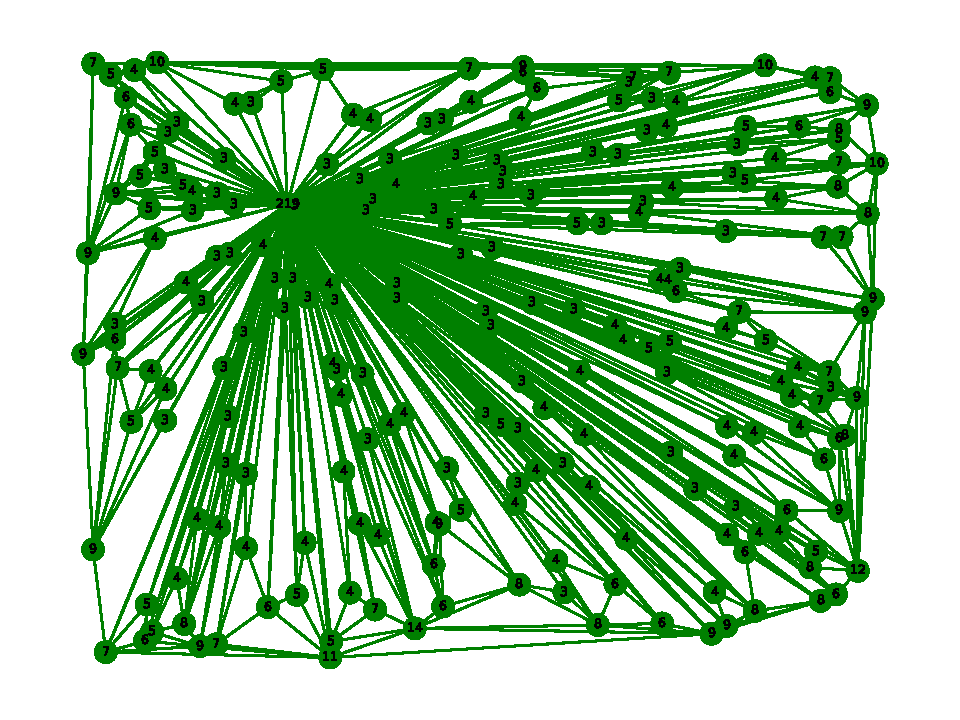
\includegraphics[width=0.6\linewidth]{figures/beamer/220.pdf}
\end{figure}  
\end{frame}

\begin{frame}{Fazit}
   \begin{figure}[h]
    \centering
    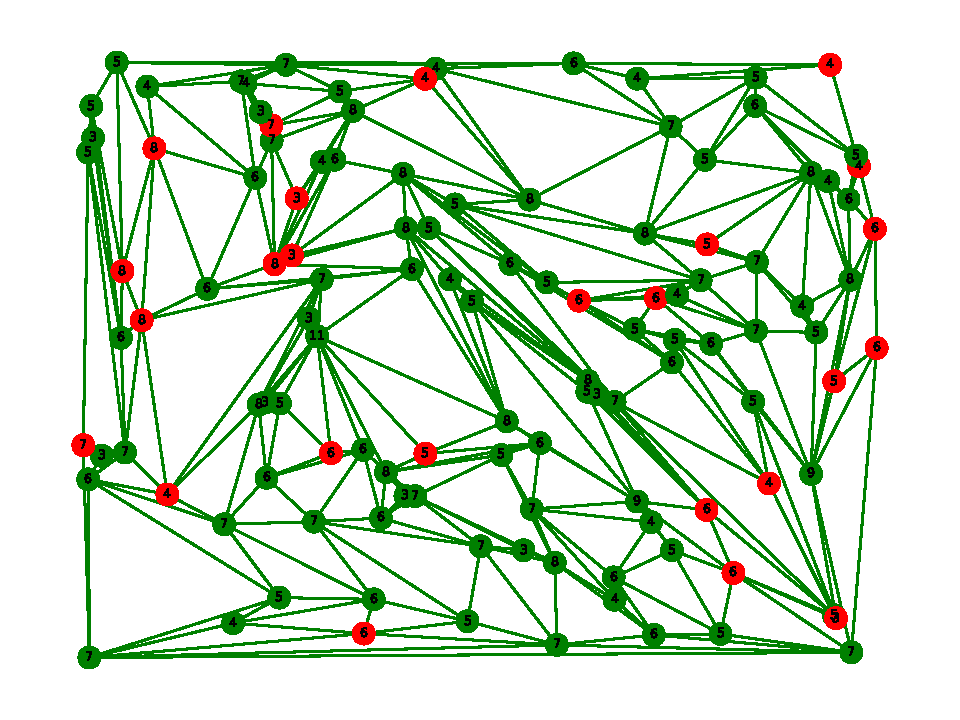
\includegraphics[width=0.6\linewidth]{figures/beamer/97.pdf}
\end{figure}  
\end{frame}

\begin{frame}{Fazit}
   \begin{figure}[h]
    \centering
    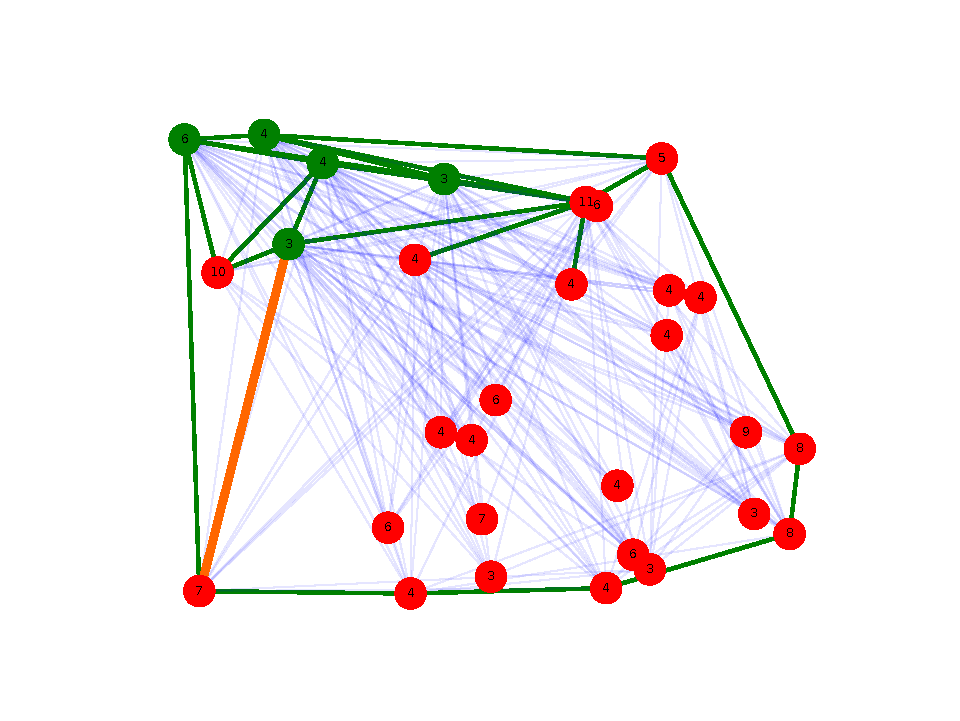
\includegraphics[width=0.65\linewidth]{figures/beamer/propergationMitLine.pdf}
\end{figure}  
\end{frame}






\section{Ausblick}
\begin{frame}{Ausblick}
    \begin{itemize}
        \item Skalierbarkeit
        \item Arbeitsspeicherverbrauch
        \item Dreiecksansatz Schwierikeit Instanzen
        \item Optimierungen Kombinationen
        \item Propergation erweitern
        \item normalverteile Triangulierung
        \item Problem abwandeln
        \begin{itemize}
            \item Kanten vorgeben
            \item Polygone
        \end{itemize}
    \end{itemize}
\end{frame}
\note[itemize]{
    \item relativ kleine Knotengrößen
    \item bei groß Arbeitsspeicher haupt Problem
    \item Dreiecksansatz alle gleich schwer
    \item warum OR-Tools Kombination gut rest nicht
    \item Propergation für Isolierte Kante
    \item Instanzegenierung mit normalerverteilen Triangulierungen
    \item Abwandeln Kanten vorgeben
    \item Polygone mit und ohne Löcher
}